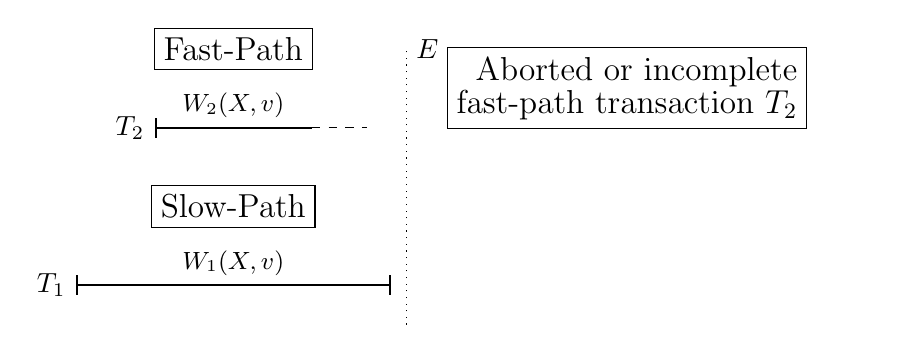
\begin{tikzpicture}
\node (w2) at (10,0) [] {};
\node (w1) at (10,-2) [] {};
\node (w3) at (18,-2) [] {};


\draw (w2) node [above] {\small {$W_2(X,v)$}};

\draw (w1) node [above] {\small {$W_1(X,v)$}};
%\draw (w1) node [below] {\tiny {$T_1$ commits}};


\node[draw,align=left] at (10,1) {{\large Fast-Path}};
\node[draw,align=left] at (10,-1) {{\large Slow-Path}};

\begin{scope}   
\draw [|-,thick] (9,0) node[left] {$T_2$} to (11,0);
\draw [-,dashed] (11,0) to (11.7,0);
\draw [|-|,thick] (8,-2) node[left] {$T_1$} to (12,-2);
\draw [-,dotted] (12.2,-2.5)  to (12.2,1) node[right] {$E$};
\end{scope}
%
\node[draw,align=right] at (15,.5) {\large {Aborted or incomplete}\\ {\large fast-path transaction $T_2$}};

%
\end{tikzpicture}
